\documentclass[11pt,a4paper]{article}

\usepackage[french]{babel}
\usepackage[utf8]{inputenc}
\usepackage[T1]{fontenc}
\usepackage{lmodern}
\usepackage{microtype}
\usepackage[a4paper,margin=2.4cm]{geometry}
\usepackage{xcolor}
\usepackage{hyperref}
\usepackage{booktabs}
\usepackage{tabularx}
\usepackage{array}
\usepackage{longtable}
\usepackage{graphicx}
\usepackage{fancyhdr}
\usepackage{titlesec}

\hypersetup{
  colorlinks=true,
  linkcolor=blue!50!black,
  urlcolor=blue!50!black,
  pdftitle={Rôle de HydrologicalTwin pour la modélisation multi-échelle de la ressource en eau},
  pdfauthor={Nicolas Flipo, Simone Mazzarelli, et l'équipe de développement de HydrologicalTwin},
}

% Commandes redéfinies localement pour conserver un fichier réellement autonome.
\newcommand{\hydrot}{\texttt{HydrologicalTwin}}
\newcommand{\subt}{\texttt{subTwin}}
\newcommand{\alphaht}{\texttt{HydrologicalTwinAlphaSeries}}
\newcommand{\cwv}{\texttt{CaWaQS-Viz}}
\newcommand{\caw}{\texttt{CaWaQS}}
\newcommand{\cawversion}{3.57}
\newcommand{\cwvversion}{000.11}
\newcommand{\htversion}{000.alpha.12}
\newcommand{\eauspra}{\texttt{EAU SPRA}}
\newcommand{\important}[1]{\textbf{#1}}

\setlength{\parindent}{0pt}
\setlength{\parskip}{0.75em}

\pagestyle{fancy}
\fancyhf{}
\lhead{Hydrological Twin}
\rhead{Modélisation multi-échelle}
\cfoot{\thepage}
\renewcommand{\headrulewidth}{0.4pt}

\titleformat{\section}{\large\bfseries}{\thesection.}{0.5em}{}
\titleformat{\subsection}{\normalsize\bfseries}{\thesubsection.}{0.5em}{}

\title{Stratégie de modélisation multi-échelle de la ressource en eau basée sur \hydrot{} - \'Etat d'avancement de \alphaht{} et perspectives}
\author{Nicolas Flipo, Simone Mazzarelli}
\date{5 mai 2026}

\begin{document}

\maketitle

\begin{center}
\small\textit{Adresse projet : }\href{mailto:hydrologicaltwin@minesparis.psl.eu}{hydrologicaltwin@minesparis.psl.eu}
\end{center}

\begin{abstract}


Ce document fait le point sur la stratégie de modélisation multi-échelle de la ressource en eau qui sera adoptée dans le cadre du projet \eauspra . Elle s'appuie sur \hydrot , qui représente un changement de paradigme en modélisation hydrologique, depuis des simulations à base physique éparpillées sans stratégie jusqu'à une véritable modélisation multi-échelle de la ressource en eau positionnée dans un continuum d'espace-état. Ce continuum d'espace-état a vocation à être mémorisé et organisé par l'infrastructure \hydrot. 
 \hydrot{}  organise les applications numériques réalisées par des modèles numériques à bases physiques en les rendant traçables et reproductibles, en les reliant à leurs  données - de structures, paramétrisation, et forçage - et aux outils utilisés à chaque étape de calcul. Il permet également de décliner ces applications de manière cohérente d'une échelle régionale vers celles des territoires, puis des sites d'exploitation comme des champs captants. 
La création de \subt{}, alimentés par des extractions territorialisées ou locales et des simulations dédiées, rend possible une modélisation multi-échelle où chaque niveau reste lié au niveau parent, tout en gagnant en finesse spatiale, en richesse des processus modélisés, et en capacité d'analyse.

Une première version du package \alphaht{} est déjà disponible, avec une classe centrale \hydrot{} qui s'appuie sur les principes d'un point d'entrée unique,  et de services (ou macro méthodes)  accessibles par une API simple et lisible. Une fois les invariants de la classe stabilisés, notamment les modes d'exposition des fonctionnalités offertes par l'outil, nous poursuivrons au cours de cette année par l'ajout progressif de capacités privées plus avancées, dont la synchronisation Git, l'extraction de territoires, l'instanciation de \subt{}  par lancement de nouvelles simulations \caw{} dans de plus petits espaces géographiques, les statistiques multi-simulations, l'inférence bayésienne, la quantification des incertitudes et la sécurisation des droits de propriété des jumeaux numériques.


\hydrot{} devient ainsi un levier pour faire passer la modélisation de la ressource en eau d'une juxtaposition d'études à une véritable architecture de connaissances organisées entre les échelles, du bassin au site local, sans perdre ni la logique scientifique, ni la mémoire des calculs.  C'est aussi une brique fondamentale et élémentaire de la future plateforme \eauspra, qui permettra de faire dialoguer les jumeaux régionaux, territoriaux et locaux dans une même logique d'organisation et de gouvernance des simulations numériques.

\end{abstract}

\section*{\`A retenir}

\hydrot{} est une structure de pilotage. Son ambition n'est pas de se substituer au modèle numérique à base physique, mais de démultiplier son potentiel quantitatif et prospectif reliant  ensemble ce que les projets dispersent trop souvent : les données, les simulations, les transformations, les visualisations, les exports, afin de reproduire la conditionnalité des phénomènes locaux aux forçages à large échelle et de garantir la prise en compte des rétroactions des propriétés locales à plus large échelle. Le passage d'un jumeau régional à des \subt{} locaux ne relève plus d'une succession de copies fragiles ; il devient un chemin organisé, inscrit dans une arborescence traçable et réutilisable. Chaque échelle peut alors gagner en finesse sans perdre le lien avec les autres.

Si cette première avancée est déjà significative, les ambitions de \hydrot{} sont plus grandes encore : faire coexister plusieurs jumeaux, gérer les droits d'accès, quantifier les incertitudes, certifier la provenance des résultats, piloter une hiérarchie de jumeaux cohérents entre eux. C'est cette vision qui fait de \hydrot{} un levier pour faire passer la modélisation de la ressource en eau d'une juxtaposition d'études à une véritable architecture de connaissance organisée entre les échelles et leur positionnement dans l'espace état des données, des simulations et des résultats. Cette infrastucure mémorielle des espaces états ouvre la voie au passage à l'échelle de l'hydrologie bayésienne, capable de mieux caractériser les incertitudes, de mieux qualifier les écarts entre les simulations et les observations, et de mieux piloter les calibrations.



\begin{figure}[h]
    \centering
    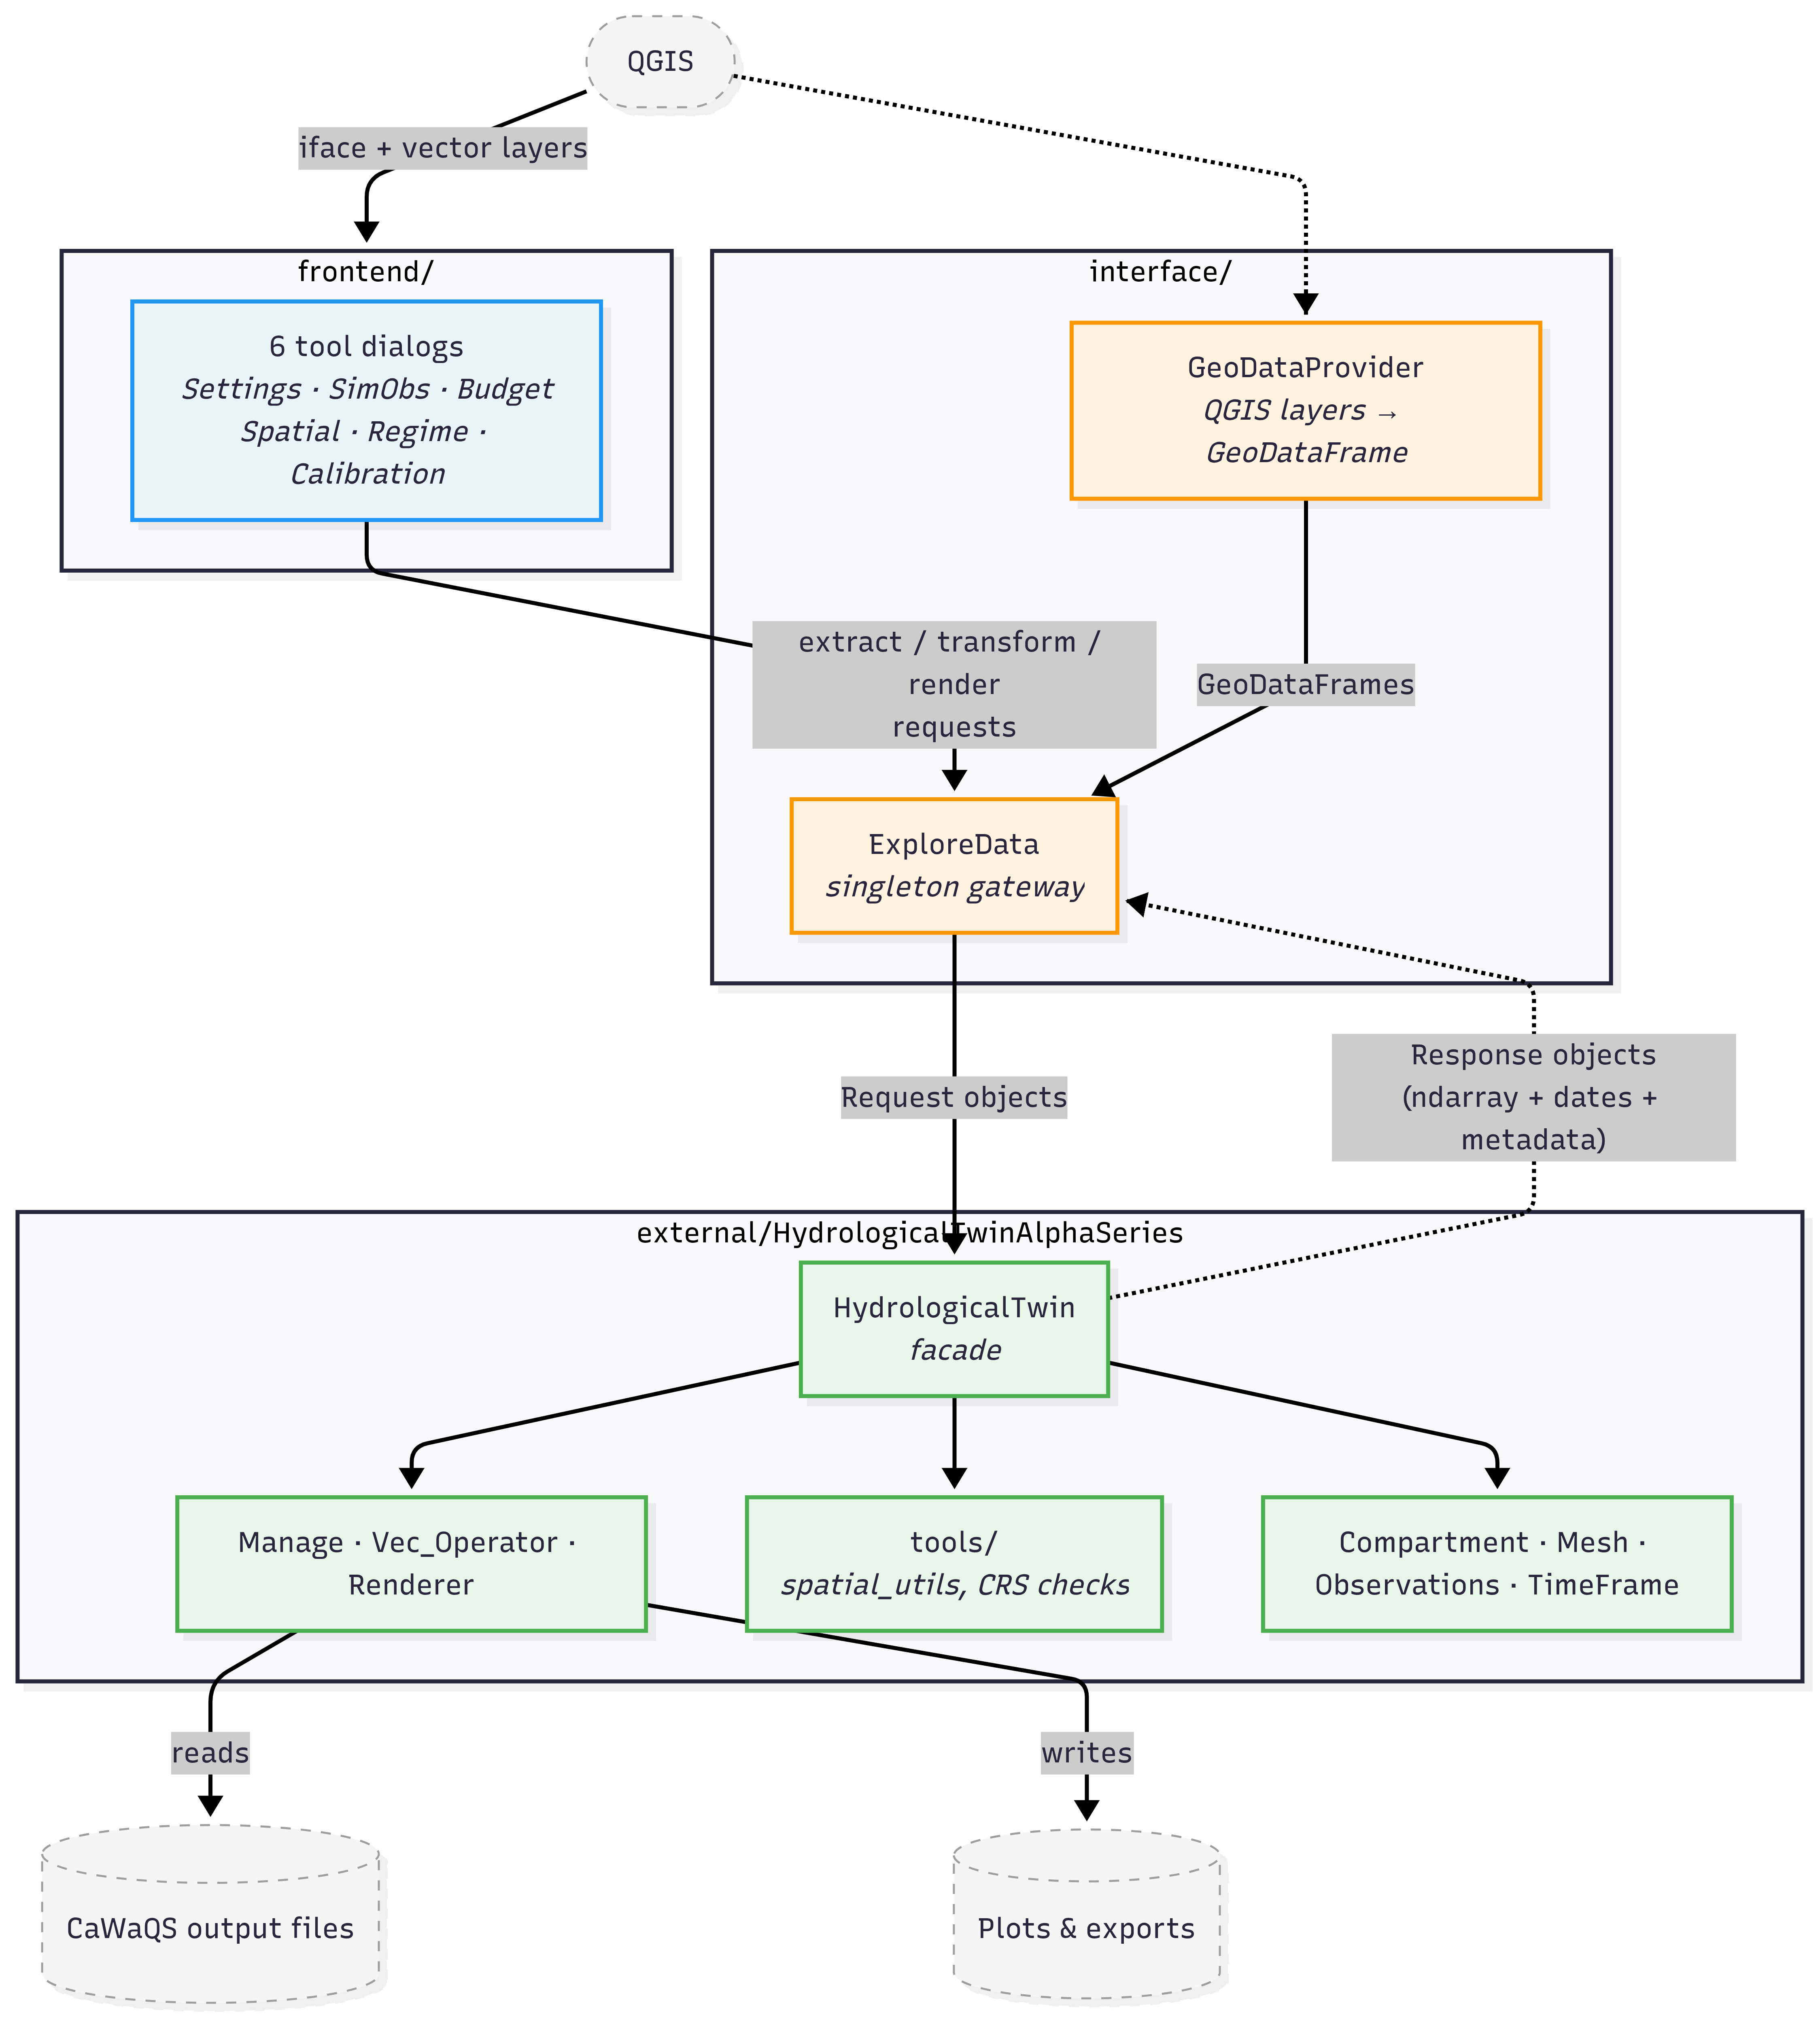
\includegraphics[width=0.8\textwidth]{Figures/Diagram_CVZ_hydrotwin.png}
    \caption{Positionnement de \hydrot{} dans l'écosystème \caw{} - \cwv}
\end{figure}


\tableofcontents

\section{\hydrot{} et la modélisation multi-échelle de la ressource en eau}

La ressource en eau se perçoit, comprend, de multiples manières. Vue de haut, elle dessine les grands ensembles continentaux et leur découpage en bassins, les tendances climatiques, les flux majeurs et les équilibres territoriaux ; approchée à une échelle intermédiaire, elle révèle les singularités d'une nappe, d'un sous-bassin, d'un tronçon de rivière ou d'un secteur de gestion ; observée enfin au plus près du terrain, elle devient affaire de captages, de zones humides, de pompages, de vulnérabilités locales, d'ouvrages et d'usages. Toute la difficulté est de faire coexister ces regards sans les laisser se séparer.

Le problème classique est que ces échelles sont souvent traitées séparément. On construit un grand modèle pour la vision régionale, puis un autre modèle local pour un besoin précis, avec des fichiers différents, des hypothèses partiellement perdues, des sorties difficilement comparables, et une traçabilité fragile.

\hydrot{} apporte une réponse structurante à cette difficulté. Il permet de conserver un fil directeur entre les échelles. Autrement dit, il donne un cadre pour passer du global au local sans casser la cohérence scientifique ni perdre la mémoire du système.

%\section{Le point de départ : un modèle à base physique a besoin d'une structure}

Utiliser un modèle hydrologique à base physique mobilise des moyens techniques et une expertise humaine. De nombreuses étapes sont nécessaires pour modéliser la ressource en eau à l'échelle régionale, comme la définition des domaines de surface et souterrain ainsi que leur découpage spatial, des forçages météorologiques, des données d'observation, des paramètres, un moteur de calcul, des sorties de simulation, puis tout un ensemble de cartes, de graphiques et d'indicateurs capables de donner forme à ce que le calcul a produit. 
Dans de nombreux projets, ces éléments existent, mais ils restent dispersés : un répertoire pour les données, un autre pour les scripts, un autre pour les sorties, parfois des traitements manuels, des conventions implicites, et \textit{in fine} une traçabilité et une reproductibilité quasiment nulles d'une simulation. 
\hydrot{}  rassemble ces éléments dans un seul objet numérique cohérent, bancarisé, synchronisé et \textit{a fortiori} pérenne. C'est précisément le sens de la description de la classe \texttt{HydrologicalTwin} dans \alphaht{} : la classe est présentée comme \og l'unique point d'entrée principal \fg{} du package. Elle encapsule tout l'état du jumeau et fournit l'API publique canonique pour la configuration, le chargement, la description, la transformation, le rendu et l'export du jumeau numérique. Il s'agit d'une véritable porte d'entrée, qui organise l'ensemble des opérations autour d'un objet métier central, plutôt que de laisser les utilisateurs naviguer dans un ensemble de scripts dispersés.

\subsection{\alphaht{} : une première étape pour stabiliser les invariants de la classe \texttt{HydrologicalTwin}}

La série Alpha correspond à une première preuve de concept publique. Elle ne contient pas encore toutes les capacités visées à long terme, mais elle montre déjà la logique d'ensemble. Comme son nom l'indique, elle est aussi un terrain d'expérimentation pour stabiliser les invariants de la classe \hydrot{} et de ses services publics, avant d'ajouter des fonctionnalités plus avancées, qui seront privées. \alphaht{} est ainsi une étape de maturation, qui permet de vérifier que les principes d'organisation du code, les modes d'exposition des fonctionnalités, les formats d'entrée et de sortie, les étapes du cycle de vie et les services publics sont bien pensés pour la suite. Il est issu de l'externalisation du backend de \cwv{}, ce qui lui confère une base solide, déjà utilisée dans un contexte opérationnel, et une logique d'organisation éprouvée. \cwv{} est une extension de QGIS qui a été développée pour rendre les résultats de \caw{} plus accessibles et plus interprétables. En externalisant le backend de \cwv{}, \alphaht{} hérite d'une expérience concrète de mise en œuvre, de gestion de données, de visualisation et d'export, qui sont des éléments clés pour la modélisation multi-échelle.

Ce premier dépôt \alphaht{} a ainsi une valeur démonstrative. Il montre que \hydrot{} n'est pas seulement une idée théorique : c'est déjà un backend autonome, distinct de l'interface cliente \cwv, avec une classe centrale nommée \texttt{HydrologicalTwin}. Pour un lecteur non informaticien, cela veut dire qu'il existe déjà un socle concret sur lequel la structuration des espaces-états des systèmes hydrologiques peut être organisée, que les étapes du cycle de vie sont déjà définies, que les services publics de base sont déjà exposés, et que la feuille de route pour les développements futurs est déjà tracée.

Le dépôt documente aussi un principe important : les opérations publiques doivent passer par des objets métier structurants, en particulier les compartiments, plutôt que par des artefacts techniques isolés. Cette manière d'organiser le code prépare naturellement la montée vers des sous-jumeaux spécialisés : on raisonne d'abord en parties du système hydrologique, puis en traitements et en sorties.

\subsection{Un cycle de vie simple à comprendre}

La classe \hydrot{} décrit un cycle de vie explicite :

\begin{center}
\texttt{EMPTY $\rightarrow$ CONFIGURED $\rightarrow$ LOADED $\rightarrow$ READY}
\end{center}

Pour une personne peu technique, ce cycle se lit presque comme une mise en route. D'abord, le jumeau existe en puissance, encore vide de tout contenu utile ; puis il reçoit sa géométrie, son projet, ses chemins de données et ses options générales ; ensuite viennent le chargement effectif des ressources nécessaires ; enfin, l'ensemble atteint un état de disponibilité où les transformations, les visualisations et les exports peuvent être produits de manière légitime.

Ce point est structurant car il impose une discipline. On ne lance pas n'importe quelle opération n'importe quand. Le jumeau sait dans quel état il se trouve et quelles actions sont légitimes à chaque étape.

\subsection{Des services publics lisibles}

La feuille de route souligne d'abord trois services publics très lisibles sur le cycle de vie : \texttt{configure}, \texttt{load} et \texttt{describe}. Une fois le jumeau dans l'état \texttt{READY}, la série Alpha met en avant trois autres familles d'action : \texttt{transform}, \texttt{render} et \texttt{export}. En langage métier, la séquence devient presque naturelle : on définit le cadre du système étudié, on ouvre réellement les données et les résultats, on regarde ce que contient le jumeau, on calcule des indicateurs ou des changements d'échelle, on produit des cartes et des vues interprétables, puis on sort les résultats vers des formats utilisables.

Même sans connaissance informatique avancée, cette organisation montre déjà ce qui fait la force de \hydrot{} : il rend pleinement explorable les simulations issues de la modélisation à base physique. Il décuple le potentiel de modèles hydrologiques comme \caw{} en offrant une interface utilisateur intuitive pour l'exploration des données, la visualisation des résultats et l'exportation des informations pertinentes. En d'autres termes, \hydrot{} transforme un modèle numérique puissant mais souvent difficile à manipuler en un outil accessible et exploitable pour les professionnels de l'eau, facilitant ainsi la prise de décision éclairée.

\section{Pourquoi cette organisation est décisive pour le multi-échelle}

Le multi-échelle ne consiste pas seulement à faire \og plus fin \fg{}. Il consiste à pouvoir passer d'une échelle à l'autre sans perdre le sens des résultats. Pour que ce voyage soit scientifiquement sûr, il faut une référence commune, une capacité d'extraction maîtrisée, la possibilité de relancer ou d'enrichir des simulations locales, et une traçabilité suffisamment robuste pour que chaque niveau demeure lisible depuis l'autre.

%\subsection{Garder une référence commune}

Le jumeau régional joue le rôle de référence. Il contient la vision d'ensemble du système : emprise spatiale, forçages, données d'observation, diagnostics globaux. Sans cette base commune, chaque zoom local risque de devenir un projet indépendant.

%\subsection{Pouvoir extraire proprement une partie du système}

Pour travailler localement, il faut isoler un sous-domaine : un sous-bassin bassin versant, un territoire objet d'un SAGE, un PTGE, une plaine alluviale, un champ captant, un champ captant porteur d'enjeu. La feuille de route de \hydrot{} identifie précisément cette étape comme un développement privé à venir : l'extraction et la synchronisation Git permettant de naviguer dans le continuum space-state des simulations. Avant même de parler de \subt , \hydrot{} prépare le terrain avec une capacité d'extraction et de navigation contrôlée pour la série Beta. C'est une étape clé pour garantir que les sous-jumeaux locaux sont bien des déclinaisons du jumeau régional, et non des projets séparés.

\subsection{Relancer ou enrichir des simulations locales}

L'enjeu n'est pas seulement de découper le domaine et de le remailler. Il faut aussi pouvoir alimenter une simulation locale avec des informations issues du jumeau parent : états initiaux, conditions aux limites, sélections de variables, paramètres hérités ou adaptés.

C'est exactement le sens de la transition annoncée entre la série Beta et le premier POC complet : créer des méthodes privées d'instanciation de \subt , permettant d'initialiser un sous-jumeau à partir d'une simulation \caw{} d'une extraction locale pure du jumeau hydrologique original sur un sous-domaine particulier.

\subsection{Conserver la traçabilité entre les niveaux}

Le bénéfice scientifique majeur de \hydrot{} est ici. Le sous-jumeau local n'est pas une copie oubliée dans un coin du disque. Il reste rattaché à son parent par la provenance des données, des logiciels, des simulations et des choix de construction. Cela change profondément la manière de faire de la modélisation locale : on ne repart pas de zéro, on spécialise proprement un objet déjà cohérent. Un \subt{} peut être compris comme une déclinaison locale du jumeau régional.

\section{Comment comprendre simplement la notion de \subt{}}

On peut comparer \hydrot{} à un atlas complet de la ressource en eau. Le jumeau principal en serait le volume entier, celui qui donne le cadre général, les continuités, les repères et la géographie d'ensemble. Le \subt{}, lui, ressemblerait à une carte détaillée consacrée à une zone particulière : plus précise, plus proche du terrain, mais toujours produite à partir du même atlas et selon les mêmes règles de lecture. Ce n'est donc ni une simple découpe géographique, ni un modèle indépendant. C'est un objet spécialisé, hérité, renseigné, et potentiellement enrichi.

%\subsection{Ce que le \subt{} permet concrètement}

Un \subt{} permettra ainsi de travailler sur un domaine local avec une résolution ou un paramétrage mieux adaptés, d'y injecter des connaissances plus fines disponibles à l'échelle du site, de tester des hypothèses particulières sans rompre le lien avec le cadre régional, de mieux distinguer ce qui relève du comportement général du bassin de ce qui appartient à une singularité locale, et, au fil du temps, de construire une hiérarchie cohérente de jumeaux qui se répondent.

%\subsection{Pourquoi c'est structurant}

Sans \hydrot{}, la création d'un modèle local dérivé d'un modèle global repose souvent sur des opérations artisanales : copie de fichiers, extraction manuelle, retraitements intermédiaires, renommages, conventions de projet implicites. Ces opérations sont possibles, mais elles sont fragiles.

Avec \hydrot{}, le passage au local devient un changement d'état organisé, inscrit dans une feuille de route explicite, et soutenu par des fonctionnalités dédiées. 

\section{De la série Alpha au multi-échelle complet : feuille de route}

La feuille de route de la classe \texttt{HydrologicalTwin} est particulièrement claire. Elle peut se lire comme une stratégie en quatre temps, où chaque étape prépare la suivante.

\subsection{Étape 1 -- Alpha : rendre le jumeau manipulable}

La première étape consiste à disposer d'un point d'entrée unique et de services lisibles. C'est la fonction de la série Alpha. Elle montre qu'un jumeau hydrologique peut être configuré, chargé, décrit, transformé, visualisé et exporté de manière cohérente. Cette étape peut sembler modeste, mais elle est fondamentale : avant de raffiner une architecture, il faut stabiliser son socle.

\subsection{Étape 2 -- Beta : préparer la navigation contrôlée}

La transition Alpha-Beta est décrite comme le développement de méthodes privées de synchronisation Git et d'extraction. C'est la construction de l'espace-état par synchronisation des savoirs et des outils de calcul. En effet pour positionner une instance de \hydrot{} dans l'espace-état, il faut pouvoir identifier exactement les données et les codes mobilisés, naviguer dans les différents états d'un projet, extraire une partie pertinente du système sans rompre la cohérence et, surtout, retrouver sans ambiguïté l'origine d'un résultat local. La synchronisation dans le continuum espace-état apporte cette mémoire du système. Elle compose la colonne vertébrale documentaire et scientifique de l'approche multi-échelle.

\subsection{Étape 3 -- Premier POC complet : instancier des \subt{}}

La transition Beta vers le premier POC complet est explicitement dédiée à la création de \subt{}. C'est le moment où \hydrot{} devient réellement un outil de modélisation multi-échelle. Le principe annoncé est fort : initialiser un sous-jumeau à partir d'une simulation du jumeau originel, mais seulement sur l'extraction locale pertinente. Cela veut dire que le modèle global fournit le contexte et les conditions héritées, que le domaine local n'est pas défini arbitrairement mais extrait du jumeau parent, que le \subt{} peut ensuite recevoir ses propres simulations adaptées au problème rencontré, et que le lien parent-enfant entre jumeaux reste toujours explicite. On passe alors d'une simple visualisation multi-échelle à une véritable modélisation multi-échelle par instanciation.

\subsection{Étape 4 -- post POC : monter en maturité scientifique}

La feuille de route prévoit ensuite quatre grands développements privés : remaillage du \subt{} pour l'enrichir et améliorer sa résolution ; un cadre bayésien pour l'auto-ajustement et la quantification des incertitudes, avec gestion parallèle de multiples instances de jumeaux ; l'amélioration de la procédure de \texttt{self\_fitting} par une analyse fréquentielle conduite pas à pas ; enfin, la gestion des droits, de la propriété intellectuelle et de la certification de l'originalité des jumeaux et de leurs composants, avec suivi de leur évolution dans le continuum espace-état. Ces quatre axes prolongent directement la logique multi-échelle. Dès qu'on dispose de plusieurs jumeaux et sous-jumeaux, il faut pouvoir raffiner, comparer, calibrer, quantifier les écarts et incertitudes, gérer les versions et protéger la valeur produite.


\subsection{Synthèse de la feuille de route}

\begin{longtable}{>{\raggedright\arraybackslash}p{0.19\textwidth} >{\raggedright\arraybackslash}p{0.23\textwidth} >{\raggedright\arraybackslash}p{0.24\textwidth} >{\raggedright\arraybackslash}p{0.25\textwidth}}
\toprule
\textbf{Étape} & \textbf{Capacité principale} & \textbf{Apport pour le métier} & \textbf{Apport pour le multi-échelle} \\
\midrule
Alpha & Point d'entrée unique et services publics de base & Comprendre, charger, décrire, visualiser et exporter le jumeau & Stabilise le socle commun avant raffinement \\
Beta & Synchronisation Git et extraction privées & Retrouver l'origine exacte des résultats et préparer des découpes fiables & Rend possible le passage contrôlé du global au local \\
Premier POC complet & Instanciation de \subt{} à partir d'extractions locales et de simulations dédiées & Étudier finement une zone à enjeu sans repartir de zéro & Fonde la modélisation multi-échelle native \\
Développements suivants & Remaillage local, Bayésien, incertitudes, multi-instances, droits et certification & Fiabiliser la décision, qualifier les écarts et protéger la valeur & Permet de piloter un ensemble de jumeaux cohérents entre eux \\
\bottomrule
\end{longtable}

Pour illustrer ce tableau, prenons un exemple simple. On construit d'abord un \hydrot{} sur un grand bassin versant, avec ses simulations existantes, ses observations régionales, sa structure spatiale et les sorties utiles à la visualisation. Ce premier jumeau donne le paysage général de la ressource en eau. Puis un territoire particulier se détache, parce qu'il concentre une tension quantitative, une baisse de la piézométrie, une sensibilité écologique ou un projet d'aménagement. À partir du jumeau principal, on en extrait un domaine local cohérent. Le \subt{} est alors instancié sur cette zone : il hérite du contexte utile du parent, puis reçoit des simulations dédiées à l'échelle locale, éventuellement enrichies par un maillage plus fin, des données supplémentaires ou des hypothèses plus ciblées. Les résultats obtenus peuvent enfin être confrontés au jumeau parent afin de vérifier la cohérence d'ensemble, de repérer les secteurs où le modèle global suffit, d'identifier ceux où un raffinement structurel éclaire réellement le système, et de préparer des stratégies de calibration ou d'estimation des incertitudes plus précises. On obtient ainsi une architecture en cascade, où les échelles ne s'opposent pas mais se répondent.



\section{Caractère transformant d'\hydrot{} pour une personne métier}

Pour un gestionnaire de bassin, un hydrogéologue, un ingénieur d'études ou un décideur, l'intérêt de \hydrot{} n'est pas d'abord informatique. Il est opérationnel. Au lieu de demander : \og Où sont les fichiers de simulation ? Quelle est la bonne version ? Qui a modifié tel paramètre ? Quel script produit cette carte ? \fg{}, on dispose d'un objet qui organise les opérations. Le travail devient plus lisible, mais surtout les résultats gagnent en crédibilité parce que leur origine, leur chemin de fabrication et leur place dans l'ensemble sont mieux documentés. Dans beaucoup de projets, une étude locale est lancée comme un nouveau chantier. Avec \hydrot{}, elle peut devenir un approfondissement d'un jumeau existant.

Cette continuité est essentielle pour la gestion de l'eau, car les décisions locales ont souvent des effets plus larges, et les résultats régionaux ont souvent besoin d'être confrontés à des réalités de terrain très fines. Le \subt{} n'a pas seulement vocation à raffiner la résolution. Il peut aussi intégrer une connaissance de terrain plus riche : ouvrages, limites locales, observations supplémentaires, contraintes hydrogéologiques particulières. Il donne une place plus claire à l'expertise métier dans la chaîne de modélisation. Il ne s'agit plus d'empiler des calculs, mais d'organiser des niveaux de connaissance.



\section{Conclusion}

On peut résumer le rôle structurant de \hydrot{} en disant qu'il unifie, discipline, prépare le passage d'échelle, conserve la mémoire du système et ouvre la voie à une véritable gouvernance des modèles. Il unifie, parce qu'il donne un seul cadre aux données, aux simulations, aux transformations et aux rendus. Il discipline, parce qu'un cycle de vie explicite évite les usages prématurés ou incohérents. Il prépare le passage d'échelle, parce que l'extraction et l'instanciation de \subt{} ne sont pas des ajouts périphériques, mais des étapes inscrites dans la feuille de route. Il conserve la mémoire du système, parce que chaque niveau peut rester lié à son origine. Enfin, il ouvre la voie à une gouvernance des modèles, parce qu'il rend pensable la coexistence de plusieurs jumeaux, de plusieurs simulations et de plusieurs niveaux de droits à l'intérieur d'une même logique d'organisation.

Ainsi, \hydrot{} est structurant non seulement parce qu'il ordonne un code, mais parce qu'il ordonne une pratique scientifique et opérationnelle.



La feuille de route portée par la classe \texttt{HydrologicalTwin} de \alphaht{} plannifie dans la durée de la première phase du projet, la montée en puissance  de la modélisation hydrologique multi-échelle, inscrite dans l'espace-état nécessaire à l'inférence bayésienne et à la gestion des incertitudes. Au départ, \hydrot{} fournit un jumeau lisible, manipulable et apte à produire des transformations, des rendus et des exports. Ensuite, il prépare les briques indispensables à une gestion rigoureuse des états, des extractions et de la traçabilité. Puis il franchit une étape décisive avec l'instanciation de \subt , qui permettra de renseigner des simulations locales tout en conservant le lien avec un jumeau parent. C'est cette articulation qui fait de \hydrot{} un levier pour la modélisation multi-échelle de la ressource en eau. Le modèle à base physique n'est pas abandonné ; il est prolongé, structuré et mis en relation avec des déclinaisons locales cohérentes. En ce sens, \hydrot{} permet de passer d'une juxtaposition d'études à une architecture de connaissance organisée entre les échelles. 

C'est aussi une brique fondamentale de la future plateforme \eauspra, qui permettra de faire dialoguer les jumeaux régionaux, territoriaux et locaux dans une même logique d'organisation et de gouvernance des simulations numériques.

\end{document}